%%%%%%%%%%%%%%%%%%%%%%%%%%%%%%%%%%%%%%%%%%%%
% PRODUCING A SELF-DRIVING MODEL
%%%%%%%%%%%%%%%%%%%%%%%%%%%%%%%%%%%%%%%%%%%%

\section{Producing a self-driving model}


% probably best to more this to results section and reference here
%\begin{verbatim}
%# data: genRoad (log2 renamed)
%# commit: 1ad187d4bff5b6936c065a1aaa15a654ef4d368c
%$ python train.py --model=sanity --outdir=../trained_models
%\end{verbatim}
%this will create the a model in trained\_output/sanity/20201120184912\_sanity.h5
% and run as per procedure described in (TODO add reference).
More results, this time as per run 43 (\ref{app_res:43}) 3 images side by side (Figure 
 \ref{fig:tcpflow_Run43}). This was a first attempt to add rain, where the effect is added to the image presented to network. Although the procedure introduces noise to images, it is somewhat unrealistic, as rain is expected to be present on the acquired image. It is left here to document the work development.
 
\begin{figure}[ht]
 \centering 
 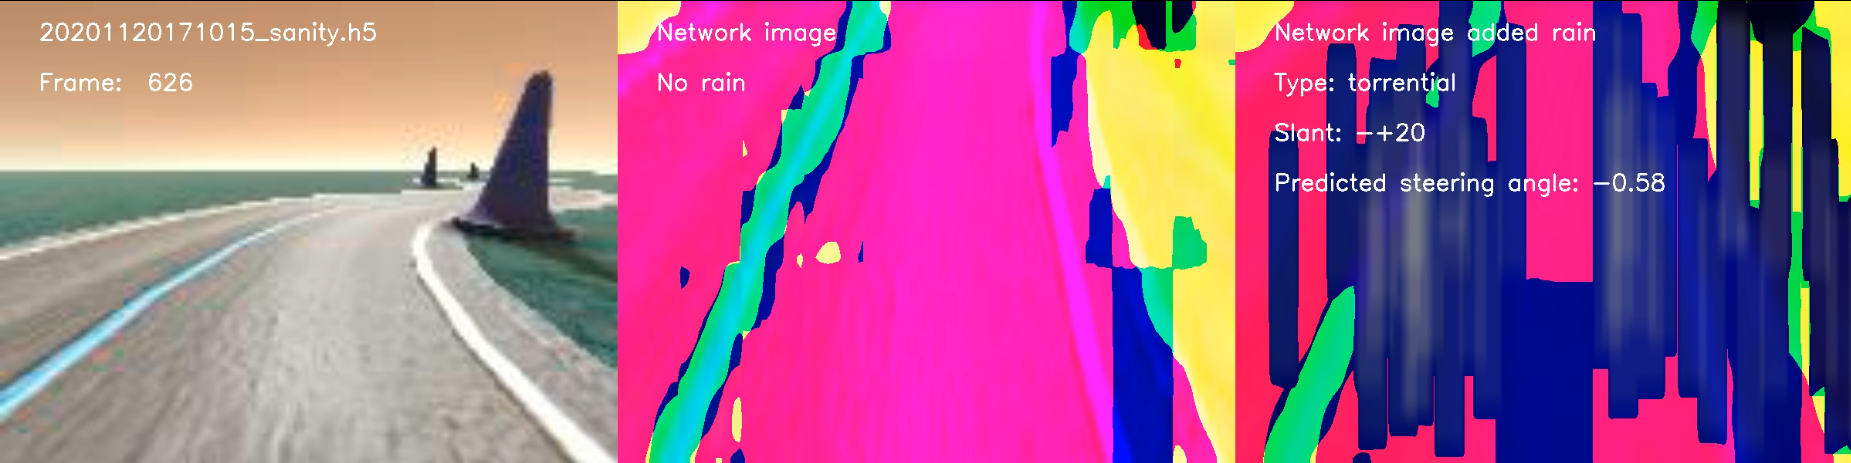
\includegraphics[width=\textwidth]{Figures/tcpflow_Run43.png}
 \caption{Video still showing torrential rain added to the image presented to the network \href{https://youtu.be/57jwwcjbfdE}{https://youtu.be/57jwwcjbfdE}}
 \label{fig:tcpflow_Run43} 
\end{figure}
%\begin{verbatim}
%# data: genRoad (log2 renamed)
%# commit: 1ad187d4bff5b6936c065a1aaa15a654ef4d368c
%$ python train.py --model=sanity --outdir=../trained_models
%\end{verbatim}
%this will create the a model in trained\_output/sanity/20201120184912\_sanity.h5
%and run as per procedure described in (TODO add reference).

\section{Producing a self-driving model}
A self-driving model that successfully drove around the Generated Track was produced 


TODO describe how SDSandbox did not work out of the box - author mentions in video "several hours of data are required" and model to nearly 24 hours to train on GPU. In practice, one augmentation and pre-processing were added, working models were produced in as little as 5 epochs of training, taking under 1m30s.
That was hard. Detail the bits that were used from TawnNet (augmentation added) and NaokiNet (crop changed). in the end two outputs were required for NaokiNet to work. Maybe move this to discussion. Here we show results.

%%%%%%%%%%%%%%%%%%%%%%%%%%%%%%%%%%%%%%%
% NETWORK TRAINING
%%%%%%%%%%%%%%%%%%%%%%%%%%%%%%%%%%%%%%%

\section{Network training and simulator testing}
\label{results:net-training} 
% write up, label runs and make reference
The first working model (able to successfully self-drive around the Generated Track) was 20201107210627\_ nvidia1.h5. A video was generated using the recording screen utility Kazam (\cite{Kazam2020}), recording at 15fps (frames per second), and published at  \href{https://youtu.be/9z0mMtOnUUc}{https://youtu.be/9z0mMtOnUUc}. Figure \ref{fig:SimTCPPred}
shows 3 stills from the video containing from left to right, the game engine, the TCP debug output and the prediction engine running.

\begin{figure}[h!]
\centering
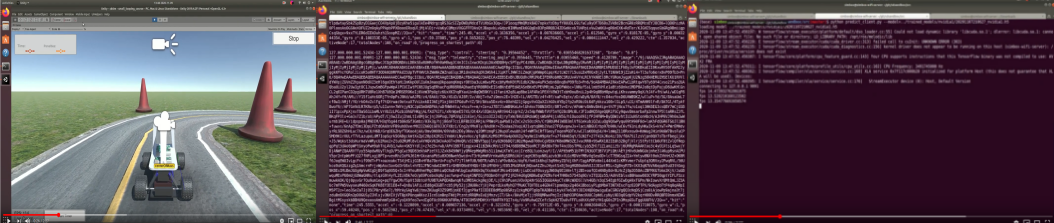
\includegraphics[width=\textwidth]{Figures/SimTCPPred.png}
\caption{Stills of video \href{https://youtu.be/9z0mMtOnUUc}{https://youtu.be/9z0mMtOnUUc} showing left to right: SDSandbox simulated car going around the Generated Track course, TCP Debug (tcpflow) and prediction engine (predict\_ client.py) running}
\label{fig:SimTCPPred}
\end{figure}

The video shows the TCP debugging, prediction engine and the game engine simulated car steering with predictions received over the TCP network. The actual code used to generate the model was not logged at the time the experiment log entry was written in the appendix log (\ref{AppendixD}). By verifying git hash commits (4 commits were made on November 7th) as documented in appendix  a second sanity check model \ref{app_res:36} (20201120171015\_ sanity.h5) was created and found to self-drive successfully around the generated track. A video was made from tcpflow frames as described at the end of \ref{app_res:36}, and uploaded to \href{https://youtu.be/JaSkkh-2xtI}{https://youtu.be/JaSkkh-2xtI}.
The video shows (fps discrepancies considered) that the \ref{app_res:36} model had a better lap around the track.
Model 37 (\ref{app_res:37}) trained with genRoad (including outliers seen in Figure \ref{fig:GeneratedRoadPlusHist}) ) did not do well. The oversteering can be seen in video \href{https://youtu.be/xGDN8qOnv9M}{https://youtu.be/xGDN8qOnv9M}. The steering angle bins and graph plots can be seen in  Figures \ref{fig:tcpflow_20201120184912_bins}  and \ref{fig:tcpflow_20201120184912_graph} in the results appendix.

% a number of runs (e.g. commit 2e5bf1b7 failed prematuraly, most failing to generate a model. Doing a diff on one of them shows that batch size was set to 128
% Could this also be an issue?
% Note in original Alexnet which we assume NVIDIA were using as a design reference, used batch size 128 for TWO channels - TODO write-up in Discussion.

%$ git diff master..2e5bf1b7 train.py | grep batch_size
%-    batch_size = conf.batch_size
%+    batch_size = conf.training_batch_size
%(base) simbox@simbox-wifi-server:~/src(master)$ git diff master..2e5bf1b7 conf.py | grep %batch_size
%+training_batch_size = 128
%-batch_size = 64
%+batch_size = 128 # nvidia1 = 64
%@@ -50,7 +49,5 @@ batch_size = 64


Another set of results for the best performing nvidia2 architecture. TODO ADD DISCUSSION, nearly steering off at large negative spike - link to video time, for three videos.  

(\url{https://youtu.be/qdTA5ho5VOE}) shows a still containing three images. The tcpflow log captured when the video was recorded provided data to plot the orange line (intensity multiplier 4, light rain) in Figure \ref{fig:sa_GeneratedTrackintensitymultiplier4_20201207091932_nvidia1}. The vehicle steers off the road and fails to turn right.


%%%%%%%%%%%%%%%%%%%%%%%%%%%%%%%%%%%%%%%%%
% DATA GATHERING
%%%%%%%%%%%%%%%%%%%%%%%%%%%%%%%%%%%%%%%%%
TODO git diff (in appendix) and itemize modifications.
    
Models are trained with code written in train.py, models.py and conf.py. This code has been modified from the original. To compare changes a git diff can be copying the original code over the source code used in this project and performing a "git diff"
\begin{verbatim}
# clone repository for dissertation
$ git clone https://github.com/dsikar/sdsandbox
# clone original
$ git clone https://github.com/tawnkramer/sdsandbox sandbox_orig
# copy original over dissertation
$ cp sandbox_org/src/* sdsandbox/src
# compare
$ cd sdsandbox 
$ git diff
\end{verbatim}


Starting with the NVIDIA baseline, a number of hyperparameters were trialed. The initial setup failed to generate usable models. 
The table below presents training results for best trained models.



Using the baseline neural network architecture as described in 
Models trained with no image pre-processing, did not perform well, leading to cars driving off the road, as shown in Fig.  sequence.

% data gathered on Robot Racing League track
We gathered 10 laps of data on the Robot Racing League track, with maximum speed set to 2.1, proportional control set to 16 and differential set to 77. Maximum steer was set to 25 (degrees). Corresponding to 12778 .jpg image files and the same number of  .json files, containing corresponding throttle and steering angle values recorded at the moment image was saved by simulator. This can be seen in the calls to Update() and SaveCamSensor functions in  
\begin{verbatim}
./Assets/Scripts/Logger.cs
\end{verbatim}